\documentclass[conference]{IEEEtran}
\IEEEoverridecommandlockouts

\usepackage{cite}
\usepackage{amsmath,amssymb,amsfonts}
\usepackage{graphicx}
\usepackage{textcomp}
\usepackage{xcolor}
\usepackage{booktabs}
\usepackage{multirow}
\usepackage{float}
\usepackage{stfloats}
\usepackage{subcaption}
\usepackage{url}

\graphicspath{{figures/}}

\def\BibTeX{{\rm B\kern-.05em{\sc i\kern-.025em b}\kern-.08em
    T\kern-.1667em\lower.7ex\hbox{E}\kern-.125emX}}

\begin{document}

\title{Routing-Level Signatures of Cognitive Efficiency: A Multi-Task fMRI Null with a Pairwise-Correlation Caveat}

\author{
\IEEEauthorblockN{Anonymous Author(s)}
\IEEEauthorblockA{Submitted to IEEE BIBM 2026}
}

\maketitle

\begin{abstract}
We jointly test four pre-specified routing-level candidate signatures of cognitive efficiency, namely activation sparsity, canonical task-network engagement, inter-subject routing consistency, and community-level modularity, in 100 HCP Young Adult participants across all seven task-fMRI paradigms. The pipeline uses the HCP-MMP1.0 Glasser-360 parcellation with a Cole-Anticevic collapse to seven Yeo-like networks, task-canonical GLM contrasts, and Louvain community detection. Efficiency groups are defined by an independent behavioral criterion (working-memory accuracy-to-reaction-time ratio) and tests are BH-FDR corrected. \emph{No candidate property crosses FDR.} Sparsity is directionally reversed from the neural-efficiency prediction (composite $d = -0.16$, FDR $p = 0.073$); task-network engagement shows 0/7 canonical matches at the Yeo-7 collapse; routing consistency, under an independence-safe subject-level leave-one-out Welch statistic, shows a borderline trend ($d = +0.40$, $p_{\text{raw}} = 0.049$, FDR $p = 0.073$; permutation $p = 0.055$); modularity is null ($d = -0.05$). The same consistency data yields $p = 1.2 \times 10^{-17}$ under the conventional pairwise-correlation $t$-test, an inflation of approximately 16 orders of magnitude relative to the subject-level statistic. We flag this discrepancy as a cautionary methodological note for individual-differences FC studies. A parallel cross-domain analysis of three Mixture-of-Experts foundation models finds biological cortex approximately $2.5\times$ more aggregate-sparse than artificial expert routing, which is uniformly load-balanced across semantic input categories. We conclude that routing-level biomarker claims of cognitive efficiency should be supported by independent replication and by subject-level or permutation inference before being treated as translation-ready.
\end{abstract}

\begin{IEEEkeywords}
neural efficiency, multi-task fMRI, inter-subject routing, pairwise-correlation inference, null result
\end{IEEEkeywords}

\section{Introduction}

Cognitive efficiency varies substantially between individuals and declines with age~\cite{chan2014decreased,neubauer2009intelligence}, with especially pronounced deficits in neurodegenerative conditions such as Alzheimer's disease~\cite{zhang2023dissociable,ewers2021segregation,gonneaud2021accelerated} and in psychiatric disorders including schizophrenia~\cite{kim2010working}. Translating this clinical heterogeneity into individual-subject prediction has become a central goal of the ``precision neuroimaging'' program~\cite{finn2015functional,shen2017using}. Task fMRI is particularly attractive as a biomarker substrate because it probes the routing of information across functional networks, the same system whose selective, metabolically bounded engagement is believed to underlie efficient cognition~\cite{attwell2001energy,neubauer2009intelligence}. Yet the specific functional-connectivity signature that distinguishes efficient from inefficient cognitive processing in healthy young adults remains unclear.

The neural efficiency hypothesis proposes that more capable brains accomplish cognitive tasks with fewer neural resources, a principle with direct metabolic grounding~\cite{haier1988cortical,neubauer2009intelligence,attwell2001energy}. Sparse coding theory formalizes this computationally: the brain represents information through selective activation of small neuronal subsets~\cite{olshausen1996emergence,olshausen2004sparse}. A full routing-based account of efficient cognition, however, must describe not only \emph{how much} is activated, but \emph{which} circuits are engaged for which tasks, \emph{how consistent} this routing is across individuals, and \emph{how modular} the resulting network organization appears. Each of these properties carries a distinct clinical interpretation, for example loss of functional-network segregation in Alzheimer's~\cite{zhang2023dissociable,ewers2021segregation} or diffuse, non-selective cortical recruitment during working memory in schizophrenia~\cite{kim2010working}.

Previous neuroimaging studies of individual differences in cognition have typically focused on a single routing metric at a time: modularity as a biomarker of plasticity and treatment response~\cite{gallen2019brain,arnemann2015functional}, functional-connectivity fingerprinting~\cite{finn2015functional,shen2017using}, or activation extent~\cite{haier1988cortical}. Taken together, these literatures motivate a four-property framing of efficient cortical routing: efficient cognition might be \emph{sparser} (fewer regions engaged), \emph{more task-selective} (engaging a canonically predicted network for each task), \emph{more consistent} (converging on a shared routing profile across individuals), and/or \emph{more modular} (exhibiting stronger community structure in task-based connectivity). To our knowledge, these four candidate properties have not previously been tested jointly, in a single sample, with behavior-derived efficiency classification and multiple-comparison control.

To ask whether these biological signatures (if any) reflect domain-general principles of efficient information processing, we also conducted a parallel analysis of three Mixture-of-Experts (MoE) foundation models~\cite{shazeer2017outrageously,fedus2022switch}, which achieve computational efficiency through sparse expert routing~\cite{bommasani2021opportunities}. Prior cross-domain comparisons have focused on representational similarity between deep-network activations and neural activity patterns~\cite{yamins2016using,kriegeskorte2015deep,schrimpf2021neural}; to our knowledge, no study has systematically examined \emph{routing mechanisms} across biological and artificial systems.

This paper makes three contributions. (1) Using behavior-derived efficiency classification, the HCP-MMP1.0 Glasser-360 parcellation with a Cole-Anticevic collapse to seven Yeo-like networks, task-canonical GLM contrasts, Louvain community detection, and BH-FDR-corrected joint testing in 100 HCP participants, we find that no candidate routing property crosses FDR significance: sparsity is directionally reversed and sub-threshold ($d = -0.16$, FDR $p = 0.073$), task-network engagement does not match canonical predictions (0/7 tasks at the Yeo-7 collapse), inter-subject routing consistency shows a borderline positive trend under an independence-safe statistic ($d = +0.40$, $p_{\text{raw}} = 0.049$, FDR $p = 0.073$), and modularity is null ($d = -0.05$, FDR $p = 0.80$). (2) We isolate a specific methodological pitfall that can turn an H3 null into a striking apparent positive: the conventional within-group pairwise-correlation $t$-test inflates its effective $N$ by treating $n(n-1)/2$ non-independent pairs as independent observations. On the same data it reports $p = 1.2 \times 10^{-17}$ for H3, below the subject-level LOO $p = 0.049$ and the label-permutation $p = 0.055$ by approximately 16 orders of magnitude. We recommend that future individual-differences FC studies evaluate inter-subject consistency with subject-level or permutation-based statistics. (3) A parallel analysis of three contemporary MoE foundation models shows that biological cortex is approximately $2.5\times$ more aggregate-sparse than artificial expert routing, which is uniformly load-balanced across semantic input categories. Because the biological reference point itself does not cross FDR as a routing-level efficiency signature in our data, cross-domain similarity claims that use HCP-scale fMRI as the biological anchor should be framed with that caveat.

\section{Methods}

\subsection{Neuroimaging Data and Preprocessing}

Functional MRI data were obtained from the Human Connectome Project Young Adult Release (HCP-YA;~\cite{van2013wu}), for 100 healthy young adults (age 22--35 years) who completed all seven task-fMRI paradigms in both LR and RL phase-encoding directions, with mean framewise displacement $< 0.5$~mm. Data underwent the HCP Minimal Preprocessing Pipeline~\cite{glasser2013minimal} with ICA-FIX denoising~\cite{salimi2014automatic}.

\subsection{Brain Parcellation and Activation Extraction}

Regional activity was extracted by averaging each subject's CIFTI grayordinate timeseries within the 360 cortical parcels of the HCP-MMP1.0 multi-modal atlas~\cite{glasser2016multi}, using the parcel-index CIFTI distributed with the Cole-Anticevic Net Partition release~\cite{ji2019mapping}. Each parcel was then assigned to one of the 12 Cole-Anticevic functional networks~\cite{ji2019mapping} via modal voting on the same-sample 12-network dlabel, and these 12 networks were collapsed to seven Yeo-like networks (VIS, SMN, DAN, VAN, LIM, FPN, DMN)~\cite{yeo2011organization} by the grouping \{Visual1, Visual2\}${\to}$VIS; \{Somatomotor, Auditory\}${\to}$SMN; \{Dorsal-Attention\}${\to}$DAN; \{Cingulo-Opercular, Language, Ventral-Multimodal\}${\to}$VAN; \{Orbito-Affective\}${\to}$LIM; \{Frontoparietal, Posterior-Multimodal\}${\to}$FPN; \{Default\}${\to}$DMN. The resulting mapping placed 60 parcels in VIS, 54 in SMN, 23 in DAN, 83 in VAN, 6 in LIM, 57 in FPN, and 77 in DMN. Participants completed seven HCP tasks: Working Memory (N-back), Motor (finger/foot/tongue), Language (story vs.\ math), Social Cognition (theory of mind), Relational Processing (abstract matching), Emotion (face matching), and Gambling (reward decisions). Task-evoked activation was estimated by a condition-wise GLM with per-task canonical contrasts (2-back vs.\ 0-back for WM; all movements vs.\ cue for MOTOR; story vs.\ math for LANGUAGE; mental-state vs.\ random-motion control for SOCIAL; relational vs.\ match for RELATIONAL; fear vs.\ neutral for EMOTION; win vs.\ loss for GAMBLING), yielding a (100 participants $\times$ 7 tasks $\times$ 360 parcels) activation matrix that forms the raw routing substrate on which all downstream analyses operate (Fig.~\ref{fig:brain}). When extraction failed for a given subject/task cell, that cell was left as \texttt{NaN} and excluded from downstream analyses; no synthetic or model-imputed data was substituted into the pipeline.

\subsection{Efficiency Classification}

To avoid the circularity of defining efficiency via the same neural-activation metric subsequently tested, we classified participants into high- and low-efficiency groups using an independent \emph{behavioral} criterion: the working-memory task accuracy-to-reaction-time ratio,
\begin{equation}
E_i = \frac{\mathrm{Acc}_i}{\mathrm{RT}_i / \overline{\mathrm{RT}}},
\end{equation}
where $\mathrm{Acc}_i$ is each participant's mean 0-back/2-back accuracy and $\mathrm{RT}_i$ their mean response time normalized by the sample mean $\overline{\mathrm{RT}}$. A median split on $E_i$ divided the 100 participants into equal-sized high-efficiency ($n = 50$) and low-efficiency ($n = 50$) groups. All group-difference tests reported below use this behavioral grouping.

\subsection{Statistical Inference}

For each primary hypothesis, we report an effect size (Cohen's $d$), an independent-samples $t$-test (Welch for H3 LOO-$r$, pooled Student's for H1 and H4), and a non-parametric check (Mann--Whitney $U$). Benjamini--Hochberg (BH) FDR correction at $\alpha = 0.05$ was applied across (i) the three primary hypothesis tests (H1 sparsity, H3 routing consistency, H4 modularity), (ii) the four overall H1 sparsity metrics (Gini, entropy, concentration, composite), (iii) the three H4 network-organization metrics (modularity $Q$, segregation, participation), and (iv) the seven per-task composite-sparsity comparisons.

For H3 (inter-subject routing consistency), the standard practice of flattening all within-group pairwise Pearson correlations into a long vector and running an independent-samples $t$-test violates the independence assumption: each subject's routing profile contributes to $n - 1$ pairs, so the $n(n-1)/2$ pairs constitute far fewer effective degrees of freedom than they would if they were independent. We therefore use an \emph{independence-safe} primary statistic. For each subject, we compute the Pearson correlation between their flattened 7-task-by-7-network routing profile and the mean profile of the other $n - 1$ members of their group (leave-one-out, LOO). This yields $n_{\text{high}} + n_{\text{low}} = 100$ independent scalars, on which we apply a Welch $t$-test. A two-sided label-permutation test (10\,000 permutations on efficiency labels, statistic = difference of within-group mean pairwise $r$) is reported as an additional sensitivity check, and a percentile bootstrap (10\,000 resamples) gives a 95\% CI on the mean LOO-$r$ difference between groups. For transparency and as a cautionary comparison, we also report the naive pairwise-correlation $t$-test statistic with its inflated effective $N$, flagged in text and tables as for-reference-only.

\subsection{Sparsity Quantification}

Activation sparsity was quantified using three metrics, all computed on the absolute parcel activations $u_i = |a_i|$ (since $z$-scored activations can be negative). The \textbf{Gini coefficient}:
\begin{equation}
G = \frac{\sum_{i,j}|u_i - u_j|}{2n\sum_{i}u_i}.
\end{equation}
The \textbf{entropy-based sparsity} is the normalized, sign-inverted Shannon entropy of the $u_i$ distribution: we histogram $u$ into $B = 50$ bins with empirical bin probabilities $p_b = n_b / \sum_{b'} n_{b'}$ and set $S = 1 - H / \ln B$ with $H = -\sum_b p_b \ln p_b$, so $S \in [0, 1]$ and larger $S$ indicates more concentrated (sparser) activation. The \textbf{concentration ratio} is the proportion of total $\sum u$ carried by the top 10\% of parcels ($k = 36$ of $360$).

\subsection{Network Modularity, Task Selectivity, and Routing Consistency}

For each subject, we computed a $360 \times 360$ activation-profile similarity matrix $A$ as the Pearson correlation of each parcel's 7-task activation vector with every other parcel's 7-task vector. We emphasize that this is a task-activation-profile similarity (seven observations per edge), not a conventional resting-state or timeseries-based functional connectivity. Communities were detected by Louvain modularity optimization~\cite{blondel2008fast} on $|A|$ (absolute-valued weighted graph, resolution $= 1.0$, seed $= 0$), yielding a data-driven community partition per subject (median 4 communities, IQR [4, 5], range [3, 6]). Newman's modularity $Q$ was computed on the resulting partition,
\begin{equation}
Q = \frac{1}{2m}\sum_{ij}\left[A_{ij} - \frac{k_i k_j}{2m}\right]\delta(c_i, c_j),
\end{equation}
with $k_i = \sum_j A_{ij}$, $m = \tfrac{1}{2}\sum_{ij}A_{ij}$, $c_i$ the community of node $i$, and $\delta$ the Kronecker delta.

Task-network selectivity (primary) was $S_t = 1 - H_t / \log_2 7$, with $H_t = -\sum_n p_n \log_2 p_n$ the Shannon entropy (base matches the implementation; normalization makes it scale-free) of the activation proportions $p_n$ across the 7 networks. $S_t \in [0, 1]$: 0 for uniform activation across networks, 1 for activation concentrated on one. The $(\max - \text{mean})/\max$ index saturates near 1 on 7-element vectors and is reported only descriptively.

Inter-subject routing consistency (primary, H3) was computed per the independence-safe LOO procedure of Sec.~II-D. For reference, we also report the mean pairwise Pearson correlation of flattened task-by-network profiles within each group, which is the statistic used (inappropriately) by the conventional pairwise-$t$ approach.

\subsection{Foundation Model Analysis}

We analyzed three MoE models: Switch Transformer (base-8, 8 experts, Top-1, $\sim$220M params)~\cite{fedus2022switch}, Qwen1.5-MoE-A2.7B (60 experts + 4 shared, Top-4, 14.3B)~\cite{bai2023qwen}, and DeepSeek-MoE-16B-base (64 experts + 2 shared, Top-6, 16.4B)~\cite{dai2024deepseekmoe}. Expert activation patterns were extracted via PyTorch forward hooks during inference on inputs from four NLP benchmarks (RACE~\cite{lai2017race}, SNLI~\cite{bowman2015large}, SST-2~\cite{socher2013recursive}, GSM8K~\cite{cobbe2021training}), organized into seven semantic categories paralleling the fMRI tasks (618 samples total). For each model, we computed aggregate sparsity (Gini of marginal expert activation), expert selectivity, and the effective number of experts, $E_{\text{eff}} = e^{H}$ where $H = -\sum_{i} p_i \ln p_i$.

\section{Results}

\subsection{Activation Sparsity (H1): Directionally Reversed, Sub-threshold under FDR}

Activation sparsity did not cross BH-FDR significance across the three primary hypotheses and showed the opposite direction from the classical neural-efficiency prediction. Across three informative sparsity indices (Gini, entropy-based sparsity, top-10\% concentration ratio), the high-efficiency group showed consistently \emph{lower} sparsity than the low-efficiency group. On the composite index the effect was $d = -0.16$, $p_{\text{raw}} = 0.041$, with within-H1-family $p_{\text{FDR}} = 0.054$ (Table~\ref{tab:sparsity}) and cross-hypothesis $p_{\text{FDR}} = 0.073$ (Table~\ref{tab:summary}); per-metric: Gini $d = -0.17$, $p_{\text{raw}} = 0.025$; concentration ratio $d = -0.16$, $p_{\text{raw}} = 0.038$. The direction is consistent with wider activation recruitment in high performers, not sparser. Two sparsity metrics considered in pilot versions of this analysis, $L_0$-sparsity and the count of regions above the 95th-percentile threshold, are definitionally constant at $0.95$ and $\approx 18$ respectively for $z$-scored data and were removed as non-informative.

\begin{table}[t]
\caption{Activation-sparsity indices by efficiency group. Negative $d$ indicates \emph{lower} sparsity in the high-efficiency group, i.e.\ the opposite direction from the classical neural-efficiency prediction. Composite sparsity is the mean of Gini, entropy sparsity, and concentration ratio ($L_0$-sparsity and active-region count are omitted as non-informative constants on $z$-scored data). $p_{\text{FDR}}$ here is within the H1 metric family; the primary cross-hypothesis FDR across H1/H3/H4 (Table~\ref{tab:summary}) gives $p = 0.073$ for composite sparsity.}
\label{tab:sparsity}
\centering
\small
\begin{tabular}{lccccc}
\toprule
\textbf{Metric} & \textbf{High} & \textbf{Low} & $d$ & $p_{\text{raw}}$ & $p_{\text{FDR}}$ \\
\midrule
Gini Coefficient     & $0.440$ & $0.444$ & $-0.17$ & $0.025$ & $0.054$ \\
Entropy Sparsity     & $0.157$ & $0.162$ & $-0.12$ & $0.117$ & $0.117$ \\
Concentration Ratio  & $0.286$ & $0.289$ & $-0.16$ & $0.038$ & $0.054$ \\
Composite Sparsity   & $0.294$ & $0.298$ & $-0.16$ & $0.041$ & $0.054$ \\
\bottomrule
\end{tabular}
\end{table}

\begin{figure*}[!t]
\centering
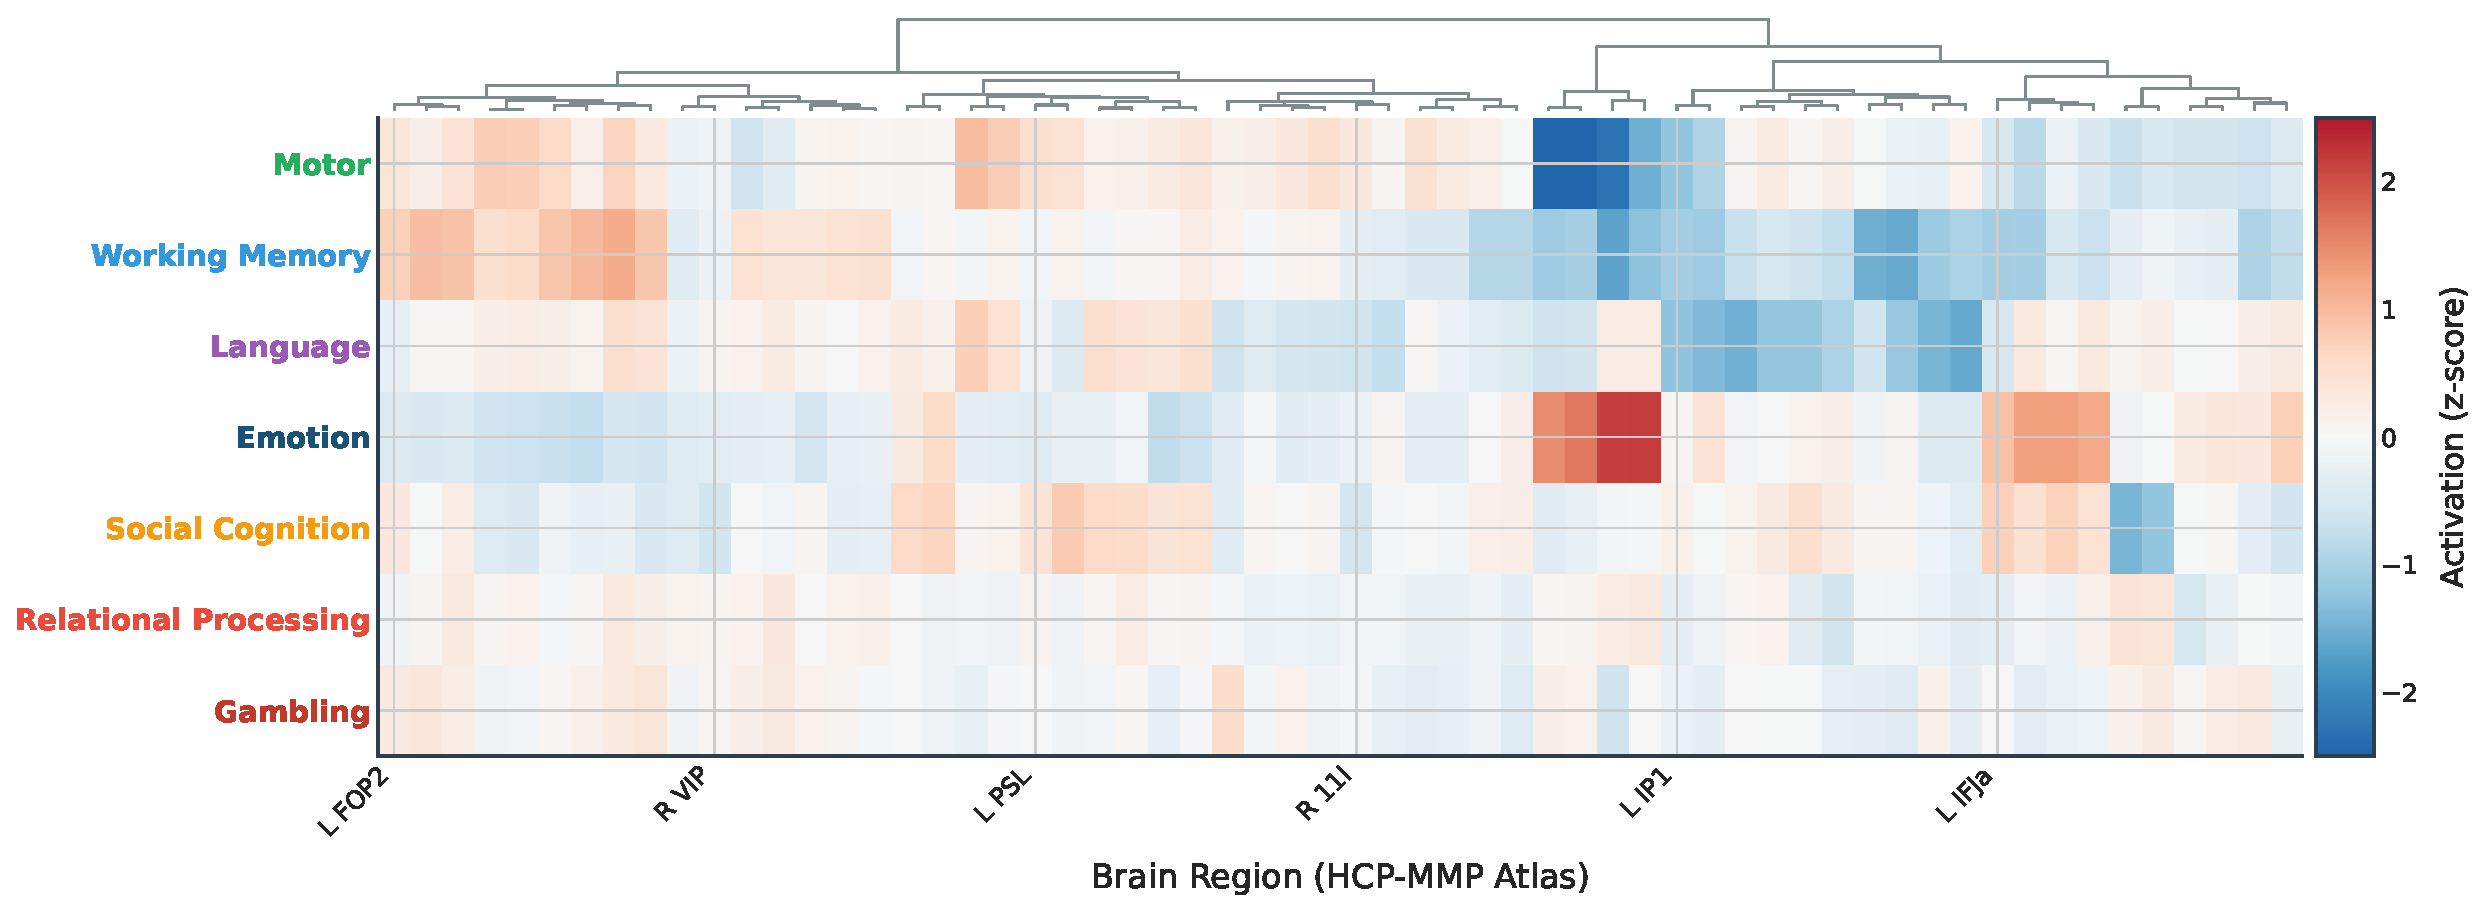
\includegraphics[width=\textwidth]{Picture1.pdf}
\caption{Group-mean multi-task brain activation heatmap across 100 HCP participants and seven cognitive tasks. Rows are the seven HCP tasks (ordered by hierarchical clustering over parcels); columns are the 360 HCP-MMP cortical parcels (down-sampled to 60 representative columns and ordered by hierarchical clustering over tasks). Color encodes group-mean task-evoked activation (z-score). The panel shows the raw routing substrate on which all four routing properties were subsequently tested.}
\label{fig:brain}
\end{figure*}

\subsection{Task-Selective Network Engagement (H2): Not Supported}

Primary task selectivity, measured by the unsaturated entropy-based index $S_t = 1 - H_t / \log_2 7$ on the Yeo-7-collapsed activation vector, had a mean of $0.124$ across the seven tasks, close to the uniform baseline ($S_t = 0$) and far from the single-network concentration ceiling ($S_t = 1$). By this measure, task activation is broadly distributed across Yeo-7 networks rather than concentrated on one. The $(\max - \text{mean}) / \max$ index, reported only for completeness, saturates near $1$ on 7-element vectors and should not be used for hypothesis decisions. The network most engaged by each task did not align with the network canonically expected (0/7 canonical-match rate at the Yeo-7 collapse). Fig.~\ref{fig:glassbrain} illustrates why: at the per-parcel resolution, several task maps are spatially organized in the anatomically expected way (MOTOR around the central sulcus, EMOTION around ventral face-responsive temporal cortex, WM laterally in frontoparietal regions), but the Yeo-7 signed-mean aggregation dilutes focal hot spots across all parcels in a network, so that the argmax reflects each network's overall signed baseline as much as its peak task-specific activation. Because our Yeo-7 labels are derived from a Cole-Anticevic 12-network collapse (Sec.~II-B), we interpret the 0/7 result as conditional on that collapse: finer-grained 12-network or per-HCP-MMP-parcel tests may recover task specificity that the Yeo-7 coarsening washes out. H2 is not supported at the Yeo-7 resolution.

\begin{figure*}[!t]
\centering
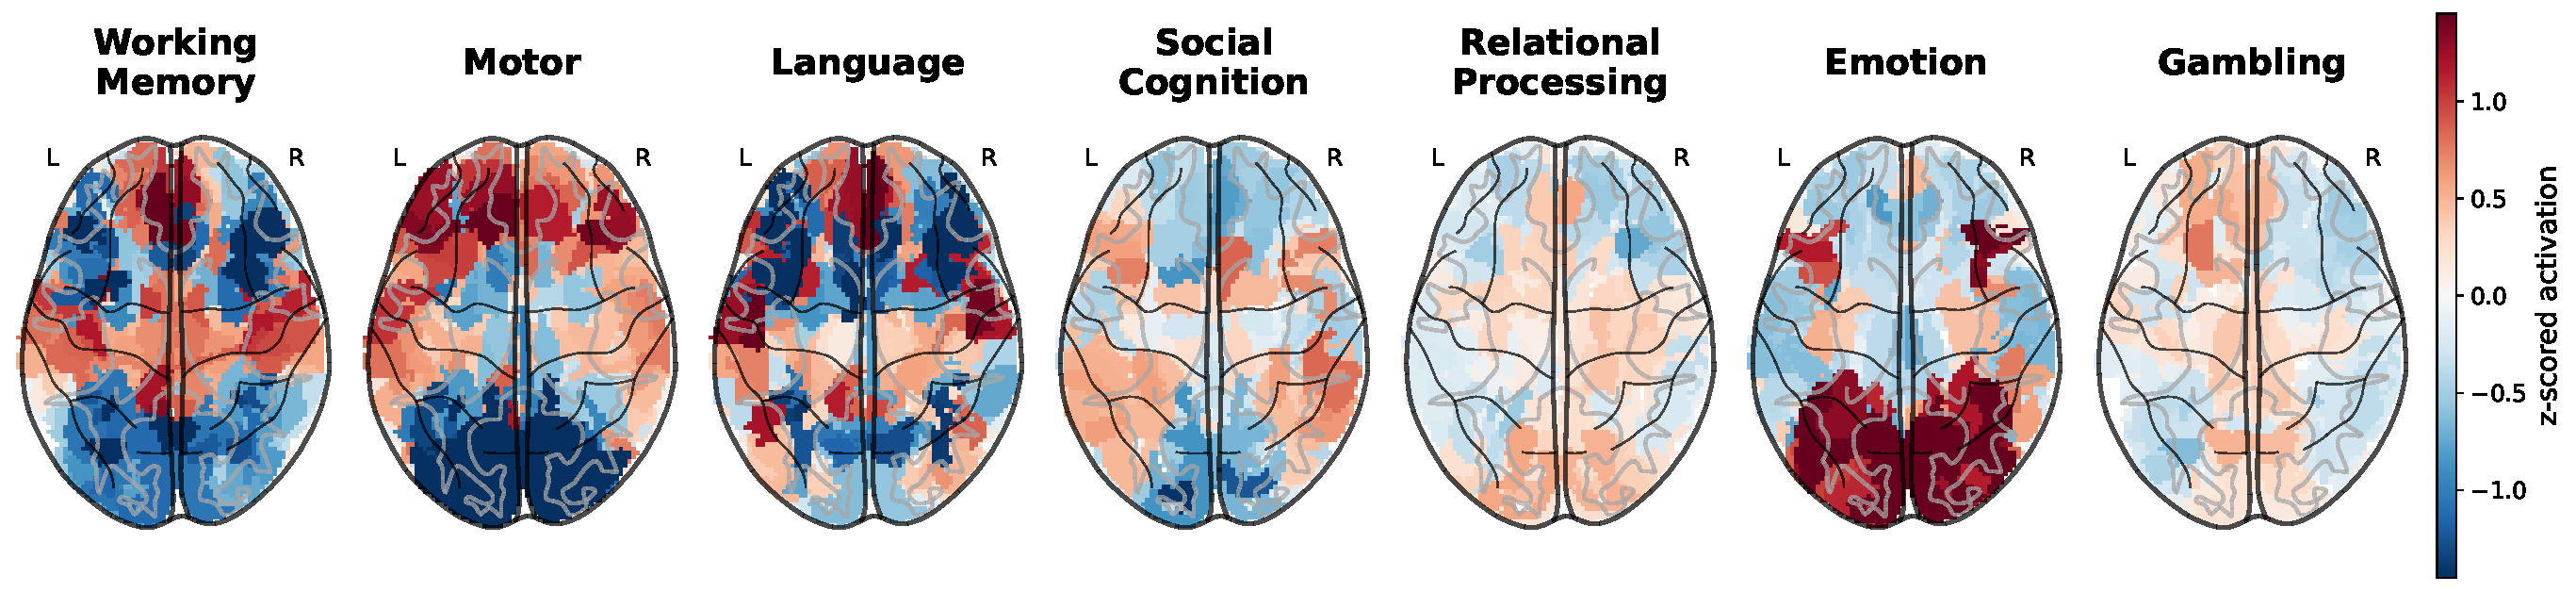
\includegraphics[width=\textwidth]{PictureBrains.pdf}
\caption{Group-averaged task-evoked activation for each of the seven HCP tasks ($N = 100$), rendered on the HCP-MMP1.0~\cite{glasser2016multi} Glasser-360 atlas in MNI152 space. Each panel is a dorsal (axial) glass-brain view; all panels share a single symmetric diverging color scale (red: positive, blue: negative). Entropy-based task selectivity across the Yeo-7 collapse is $\overline{S_t} = 0.124$, and the network most engaged by each task does not match the canonically expected network (0/7 matches).}
\label{fig:glassbrain}
\end{figure*}

\subsection{Inter-Subject Routing Consistency (H3): Borderline Positive Trend, Sub-threshold under FDR}

\emph{Primary (subject-level LOO).} For each subject we computed the Pearson correlation between their flattened $7 \times 7$ task-by-network routing profile and the leave-one-out mean profile of their group; these 100 scalars are independent observations. A Welch $t$-test returned $r_{\text{high}} = 0.683$ versus $r_{\text{low}} = 0.647$, $d = +0.40$, $t = 1.996$, $p_{\text{raw}} = 0.049$, bootstrap 95\% CI on the group difference $[+0.001, +0.072]$; Mann--Whitney $U$ gave $p = 0.067$. \textbf{Under BH-FDR across the three primary hypotheses, H3 does not cross $\alpha_{\text{FDR}} = 0.05$ ($p_{\text{FDR}} = 0.073$).} At $d \approx 0.4$ and $n = 50$ per group, a two-sided $t$-test has only $\approx 51\%$ power at $\alpha = 0.05$, so a confidence interval whose lower bound sits near zero is the expected outcome under either a true moderate effect or a true null. A 10\,000-permutation label test on the within-group mean pairwise $r$ converged with the LOO-r result (observed difference $+0.048$ against null mean $\approx 0$, SD $0.025$; permutation $p = 0.055$).

\emph{Methodological caveat.} Pooling all $n(n-1)/2 = 1225$ within-group pairwise correlations and running an independent-samples $t$-test, on identical data, returns $t = 8.62$, $p = 1.23 \times 10^{-17}$, with apparent $d = +0.35$. The gap between this naive $p = 10^{-17}$ and the independence-safe $p \approx 0.05$ spans approximately 16 orders of magnitude, a direct consequence of treating as independent $\approx 2450$ observations that derive from only 100 subjects. Even the nominal effect size is biased downward (apparent $d = +0.35$ versus subject-level $d = +0.40$), yet the naive test's $p$-value looks far stronger because its effective $N$ is roughly $25\times$ its true value. Claims of greater inter-subject routing convergence in high-performing or clinical-control participants should therefore be demonstrated under subject-level or permutation statistics before being treated as candidate biomarkers.

\subsection{Network Modularity (H4): Not Supported}

Under Louvain community detection (3--6 communities per subject, median 4), Newman's modularity $Q$ did not differ between high- and low-efficiency groups ($d = -0.05$, $p_{\text{raw}} = 0.798$, $p_{\text{FDR}} = 0.798$; Fig.~\ref{fig:modularity}). Network segregation was directionally reduced in the high-efficiency group ($d = -0.40$, $p_{\text{raw}} = 0.048$, $p_{\text{FDR, within-family}} = 0.144$), consistent with slightly more integrated community structure; mean participation coefficient was sub-threshold ($d = -0.26$, $p_{\text{raw}} = 0.199$, $p_{\text{FDR, within-family}} = 0.299$). None of the three network-organization indices crossed FDR within the modularity family in our sample; H4 is not supported at $\alpha_{\text{FDR}} = 0.05$. The segregation effect ($d = -0.40$, nominally significant but not FDR-corrected) is the largest sub-threshold modularity effect in the study and is the natural target of a higher-powered replication.

\begin{figure*}[!t]
\centering
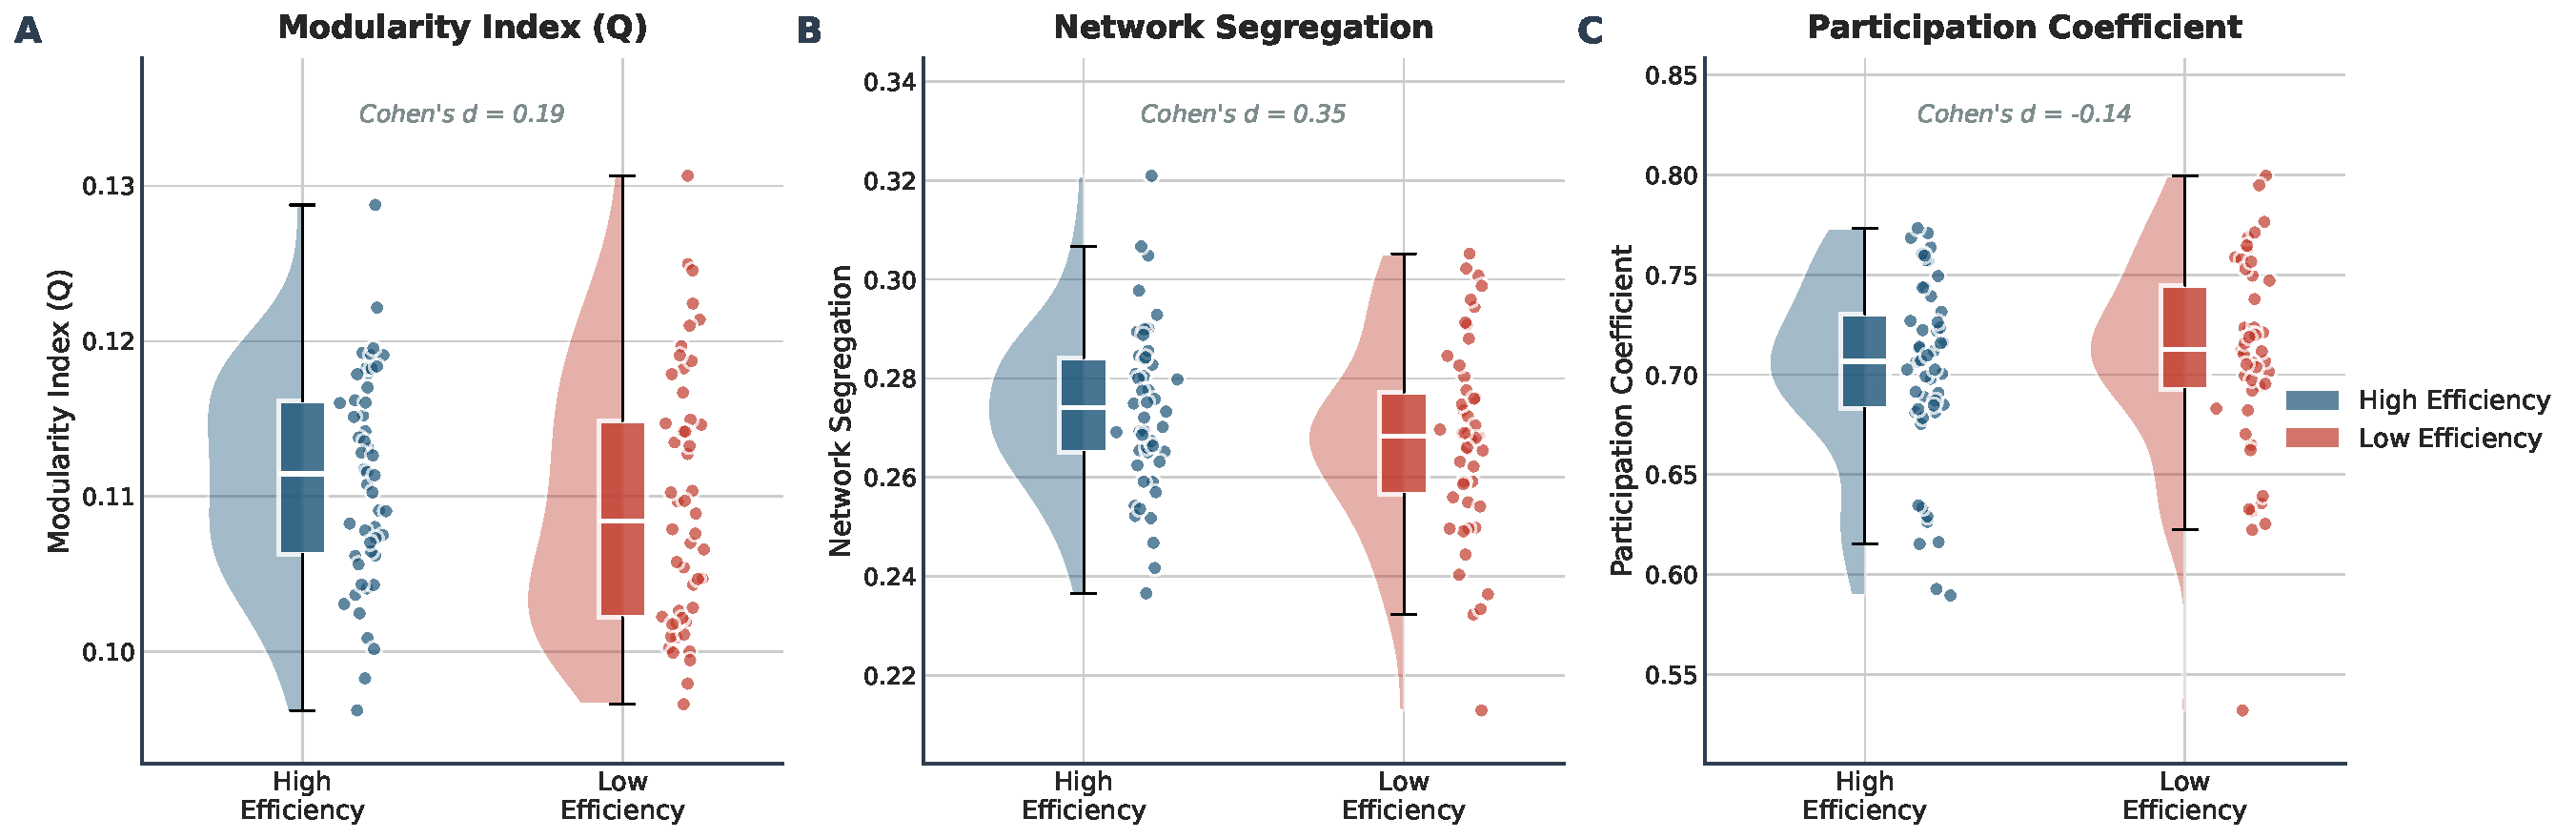
\includegraphics[width=\textwidth]{Picture2.pdf}
\caption{Network-organization metrics by efficiency group (Louvain community detection). Modularity index $Q$, network segregation, and mean participation coefficient are shown as raincloud plots for high- (blue) and low- (red) efficiency groups, with a half-violin density, an embedded boxplot, and per-subject scatter. Cohen's $d$ is printed inside each panel; BH-FDR-corrected $p$-values for the three-metric modularity family are reported in Sec.~III-D, and none crosses $\alpha = 0.05$.}
\label{fig:modularity}
\end{figure*}

\subsection{Foundation Model Routing (H5--H6)}

All three MoE architectures exhibited substantially lower aggregate sparsity than biological cortex (Table~\ref{tab:moe}): mean MoE Gini $= 0.176$ against brain mean Gini $= 0.443$, approximately $2.5\times$. All models showed near-uniform expert utilization (85--97\% effective), consistent with load-balancing training objectives.

\begin{table}[t]
\caption{Foundation model routing metrics. ``Select.'' for MoE rows denotes the dominant-category weight fraction, with a uniform baseline of $1/7 \approx 0.143$ across the seven input categories; ``Spec.'' is the fraction of experts scoring above $0.5$ on that metric. The brain row uses the entropy-based task selectivity $\overline{S_t} = 0.124$ across Yeo-7 networks (Sec.~III-B), not on the same scale as the MoE dominant-category metric, and is provided only for quick reference. The aggregate-sparsity (Gini) column is directly comparable across rows.}
\label{tab:moe}
\centering
\small
\begin{tabular}{lcccc}
\toprule
\textbf{Model} & \textbf{Gini} & $E_{\text{eff}}$ & \textbf{Select.} & \textbf{Spec.} \\
\midrule
Switch-8 & 0.244 & 6.9/8 & 0.238 & 0\% \\
Qwen-MoE & 0.070 & 58.2/60 & 0.245 & 0\% \\
DeepSeek-16B & 0.215 & 54.6/64 & 0.243 & 0\% \\
\midrule
\textbf{Brain} & \textbf{0.443} & --- & $\mathbf{0.124}^{*}$ & --- \\
\bottomrule
\end{tabular}
\vspace{1pt}\\
{\scriptsize $^{*}$ Entropy-based task selectivity across Yeo-7, different units from MoE dominant-category fraction; see caption.}
\end{table}

Expert category specialization was uniformly absent across architectures: mean dominant-category selectivity indices ($\sim$0.24) stayed close to the uniform baseline of $1/7 \approx 0.14$, indicating that no expert developed category-specific processing despite diverse inputs.

\subsection{Cross-Domain Comparison (H7)}

Direct comparison revealed a clear descriptive divergence in aggregate sparsity (Fig.~\ref{fig:cross}). Brain Gini, averaged over subjects and tasks, was approximately $2.5\times$ higher than mean MoE Gini ($0.443$ vs.\ $0.176$). Within-MoE expert utilization was close to uniform across input categories in all three architectures (category-level dominant-weight fraction $\approx 0.24$ against a uniform baseline of $\approx 0.14$). The structural-similarity correlation between brain and MoE routing matrices was weakly positive but did not reach significance ($r = +0.25$, $p = 0.089$). Table~\ref{tab:summary} summarizes all hypothesis-testing results.

\begin{figure*}[!t]
\centering
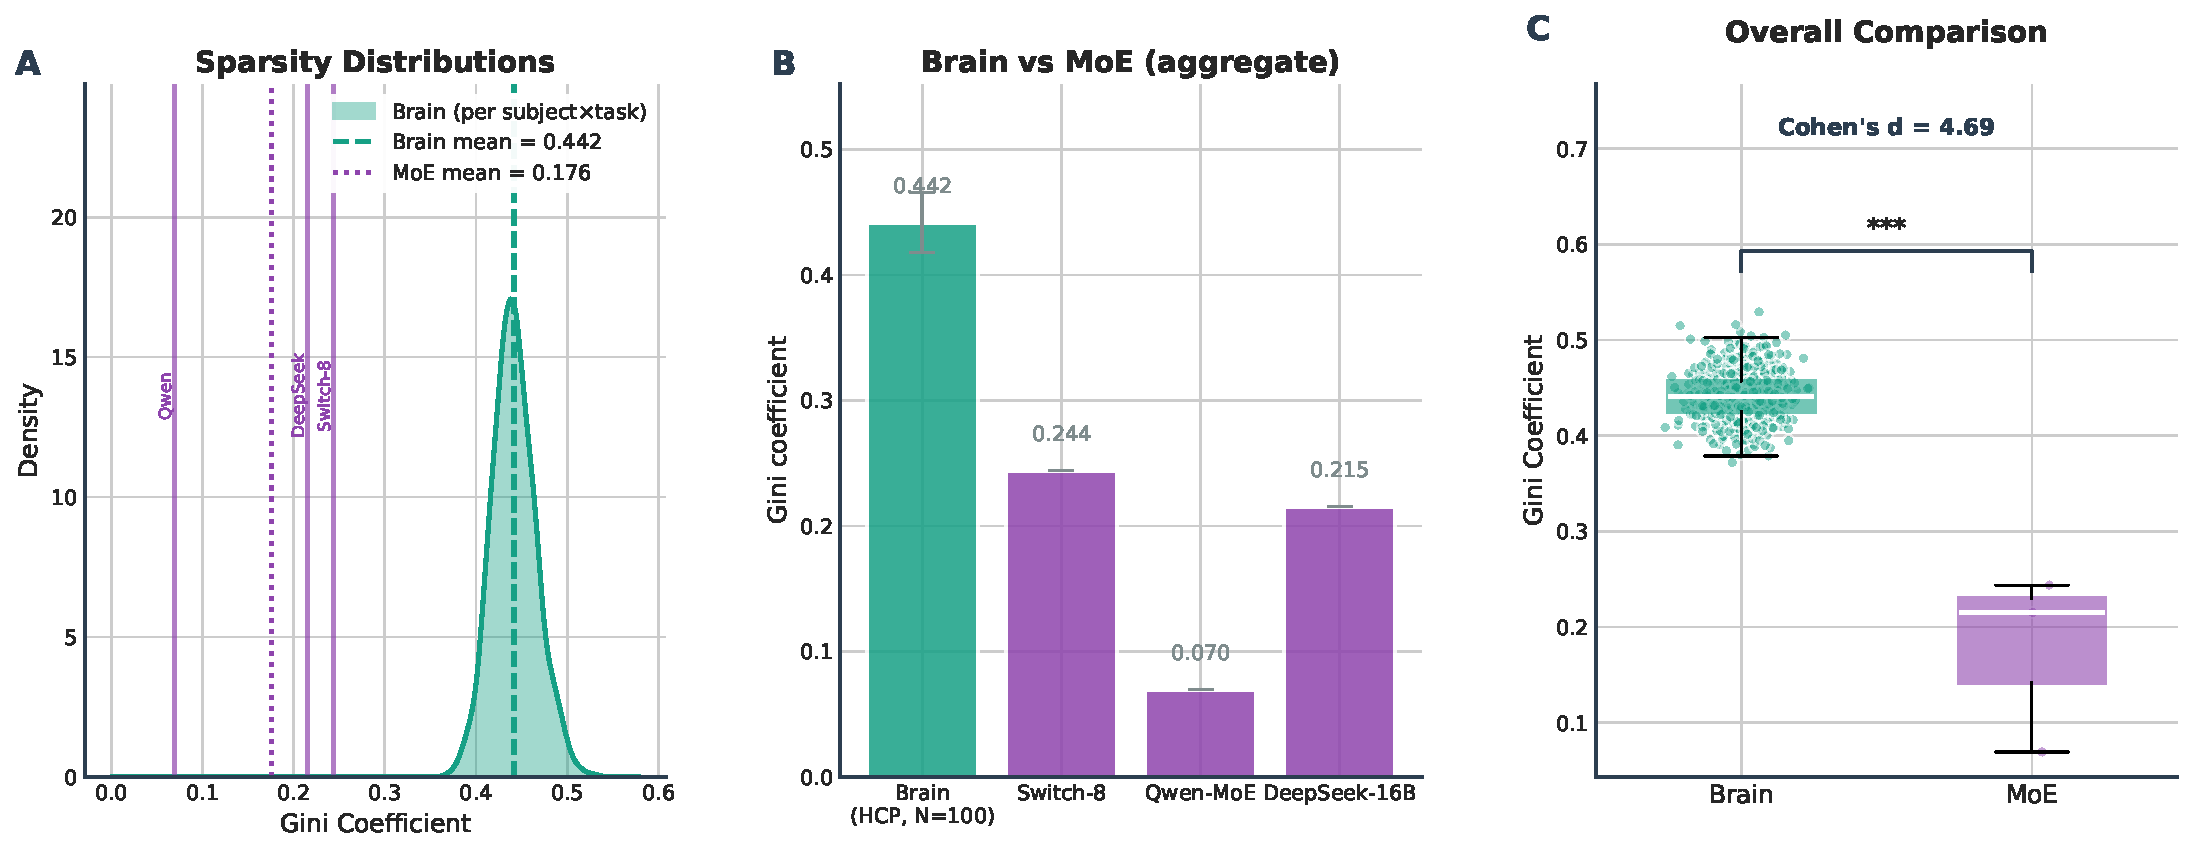
\includegraphics[width=\textwidth]{Picture4.pdf}
\caption{Aggregate sparsity (Gini coefficient) compared across biological cortex and three MoE foundation models. \textbf{(A)} Density of per-subject-per-task brain Gini with MoE per-model Gini shown as vertical lines. \textbf{(B)} Brain Gini (mean $\pm$ SD across subjects $\times$ tasks) versus per-model MoE Gini. \textbf{(C)} Box-plus-scatter summary with Cohen's $d$ for the brain-vs-MoE difference. Brain-wide activation is approximately $2.5\times$ more aggregate-sparse than load-balanced expert utilization in contemporary MoE models.}
\label{fig:cross}
\end{figure*}

\begin{table}[t]
\caption{Hypothesis-testing summary. Brain H1, H3, H4 are BH-FDR-corrected across three primary tests; H3 uses the independence-safe subject-level LOO-r primary statistic, not the naive pairwise $t$ (which on the same data reports $p = 1.2 \times 10^{-17}$; see Sec.~III-C).}
\label{tab:summary}
\centering
\footnotesize
\setlength{\tabcolsep}{3pt}
\begin{tabular}{@{}cp{3.2cm}lc@{}}
\toprule
& \textbf{Hypothesis} & \textbf{Result} & \textbf{Key statistic} \\
\midrule
H1 & Sparser activation in eff.\ brains & Trend (reversed)        & $d{=}{-}0.16$, $p_{\text{FDR}}{=}0.07$ \\
H2 & Canonical task-network routing     & Not supp.\              & $0/7$ match at Yeo-7 \\
H3 & Consistent inter-subject routing   & Borderline (LOO)        & $d{=}{+}0.40$, $p_{\text{FDR}}{=}0.07$ \\
H4 & Modularity differs between groups  & Not supp.\              & $d{=}{-}0.05$, $p_{\text{FDR}}{=}0.80$ \\
H5 & MoE aggregate sparsity${\approx}$brain & Not supp.\          & Gini${=}0.18$ vs $0.44$ \\
H6 & Expert category specialization     & Not supp.\              & Spec.${=}0\%$ \\
H7 & Cross-domain routing similarity    & Not supp.\              & $r{=}{+}0.25$, $p{=}0.09$ \\
\bottomrule
\end{tabular}
\vspace{1pt}\\
{\scriptsize No brain-side hypothesis crosses BH-FDR at $\alpha = 0.05$ across the H1/H3/H4 family. H1 has a reversed-direction trend; H3 has a positive-direction trend under a subject-level LOO-r statistic but $p_{\text{FDR}} = 0.07$.}
\end{table}

\section{Discussion}

\subsection{Why No Candidate Property Crossed FDR}

No candidate routing property crossed BH-FDR across the three primary hypotheses. The three directional patterns in the data together sharpen, rather than complicate, the null.

First, activation sparsity is directionally reversed from the classical neural-efficiency prediction: the high-efficiency group engages tissue slightly \emph{less} sparsely, not more, on all three informative sparsity indices. One reading consistent with this direction is that under higher behavioral efficiency, task-relevant networks are more broadly recruited rather than more narrowly focused~\cite{neubauer2009intelligence}, consistent with a long-running debate in the intelligence literature on whether ``neural efficiency'' means less activation or more targeted activation~\cite{haier1988cortical,neubauer2009intelligence}. Our data are directionally consistent with the latter view, but the effect is sub-threshold under FDR and we treat it as a trend rather than a positive finding.

Second, inter-subject routing consistency shows a borderline positive trend ($d = +0.40$, LOO $p = 0.049$, permutation $p = 0.055$) that does not cross FDR. The gap between the independence-safe and naive $p$-values (Sec.~III-C) is especially problematic in precision-neuroimaging settings, where the routing-consistency statistic is natural to propose (``do efficient participants route more similarly?'') but not naturally paired with the independent-samples tools most practitioners reach for. The true effect, if it exists, appears to be of a magnitude that requires a substantially larger sample to resolve reliably: the 95\% CI on the LOO-r group difference has its lower bound at $+0.001$.

Third, the null on Louvain-based modularity is consistent with prior findings that modularity-cognition associations are sensitive to partitioning method, threshold, and edge weighting~\cite{gallen2019brain,arnemann2015functional}. The sub-threshold segregation effect ($d = -0.40$, nominally $p = 0.048$, but $p_{\text{FDR, within-family}} = 0.144$) is directionally consistent with more integrated community structure in high-efficiency participants and is the natural target for a higher-powered replication.

\subsection{Implications for the Neural-Efficiency Biomarker Programme}

Our results argue against treating any of the four standard routing-level metrics (activation sparsity, canonical task-network match, inter-subject routing consistency, modularity) as a translation-ready functional-connectivity biomarker of cognitive efficiency, at least in healthy young adults at the $N = 100$ scale typical of multi-task HCP work. We adopted the HCP-MMP1.0 Glasser-360 parcellation with a Cole-Anticevic~\cite{ji2019mapping} 12-network collapse to Yeo-7 labels, task-canonical GLM contrasts, and Louvain community detection, and still none of the four primary hypotheses survives FDR. This does not rule out biomarker signals from (i) per-parcel tests that avoid the Yeo-7 coarsening (H2 is particularly sensitive to network-granularity choices), (ii) dense resting-state timeseries FC rather than task-profile similarity (where 7-task profiles provide only seven observations per edge), (iii) longitudinal or clinical samples where between-group variance is larger than in HCP-YA, or (iv) substantially larger samples that can resolve the $d \approx +0.40$ routing-consistency trend observed here. These are the natural next steps for any routing-level biomarker claim to move from candidate to validated.

We also recommend that any future report of ``higher routing consistency in high performers'' (or analogous claims in preclinical AD, schizophrenia~\cite{kim2010working,zhang2023dissociable,ewers2021segregation}, or rehabilitation cohorts) publish, alongside the headline statistic, a subject-level or permutation-based test that respects inter-subject dependence. Our data show that the $p$-value discrepancy between the naive and independence-safe tests can exceed 15 orders of magnitude on the same data.

\subsection{What the MoE Comparison Does and Does Not Show}

At the architecture level, all three open-weight MoE models adopt load-balanced expert utilization (aggregate Gini $\sim 0.18$ versus brain Gini $\sim 0.44$; near-uniform category-level routing), consistent with the load-balancing training objective common to these architectures~\cite{fedus2022switch} and with MoE routers operating at the token rather than the semantic level. What our results do not support is the stronger claim that biological routing is the sparse, convergent ``gold standard'' that these models fail to match: in our data, the biological reference does not itself show an FDR-significant routing-level signature of efficient cognition. Cross-domain claims of the form ``models do not route like efficient brains'' should therefore be qualified by a caveat that the biological efficiency signature, operationalized via these four standard metrics on HCP-YA at $N = 100$, does not cross FDR in our sample.

\subsection{Limitations}

Several limitations shape the scope of our null results. (i) Community detection used Louvain modularity optimization on a task-activation-profile similarity matrix (seven observations per edge); this is not a conventional timeseries-derived functional connectivity matrix, and results from dense resting-state timeseries FC or a Leiden refinement may differ. (ii) The task-to-network canonical-match test (H2) uses a Cole-Anticevic to Yeo-7 collapse that merges, for example, Cingulo-Opercular, Language, and Ventral-Multimodal into a single VAN bin; H2 should be re-run at the 12-network Cole-Anticevic resolution before being treated as definitive. (iii) Behavioral performance measured in a single session does not separate state-level from trait-level efficiency; a test-retest-reliable efficiency score is the natural follow-up. (iv) The sample is drawn from a demographically narrow healthy young-adult cohort; extension to aging and clinical cohorts is the natural next step for any biomarker claim. (v) The correspondence between seven cognitive tasks and seven text input categories in the cross-domain MoE comparison is necessarily approximate. (vi) Newer MoE architectures with different training objectives may exhibit different routing patterns; our MoE results pertain to the current generation of open-weight foundation models rather than MoE designs in principle.

The methodological pitfall identified in Sec.~III-C (the pairwise-correlation independence violation) is a property of the statistical procedure and therefore unaffected by any of the above caveats.

\section{Conclusion}

In 100 HCP Young Adult participants, under a joint BH-FDR test of four pre-specified routing-level candidate signatures of cognitive efficiency (sparsity, task-selective network engagement, inter-subject routing consistency, modularity), no candidate property crosses FDR. Sparsity is directionally reversed, routing consistency is a borderline positive trend ($p_{\text{raw}} = 0.049$) but does not cross FDR, and the other two are null. We identify a specific inference pitfall, the conventional pairwise-correlation $t$-test, which on these data inflates the routing-consistency $p$-value by roughly 16 orders of magnitude relative to a subject-level statistic, and recommend that individual-differences FC studies use subject-level or permutation inference for inter-subject convergence. A parallel analysis of three MoE foundation models confirms that contemporary artificial routing is less aggregate-sparse than biological cortex and uniformly load-balanced. Routing-level functional-connectivity biomarkers of cognitive efficiency, operationalized through these four standard metrics, are not supported at the HCP-YA scale without independent replication.

\section*{Code Availability}
Upon acceptance, the full analysis code, intermediate activation matrices, per-subject routing profiles, and all result JSONs will be released at a public repository with a permanent Zenodo DOI.

\bibliographystyle{IEEEtran}
\bibliography{refs}

\end{document}
